\documentclass[12pt,a4paper,fleqn]{article}
\usepackage[utf8]{inputenc}
\usepackage{amsmath}
\usepackage{amsfonts}
\usepackage{amssymb}
\usepackage{tcolorbox}
\usepackage{geometry}
\usepackage{hyperref}
\usepackage{enumitem}
\usepackage{graphicx}
\usepackage{fancyhdr}
\usepackage{array}   % for adjusting row height

\renewcommand{\arraystretch}{1.5} % adjust the vertical spacing between rows

% Márgenes
\geometry{top=2.5cm, bottom=2.5cm, left=2.5cm, right=2.5cm}

% Encabezado y pie de página
\pagestyle{fancy}
\fancyhead[L]{Apuntes de Derivadas}
\fancyhead[C]{}
\fancyhead[R]{\thepage}
\fancyfoot[L]{}
\fancyfoot[C]{}
\fancyfoot[R]{}

% Título
\title{Apuntes de Derivadas}
\author{Ariel Alejandro Calderón}
\date{\today}

\begin{document}

\maketitle

\newpage
\tableofcontents
\newpage

\section{Derivadas}

% Ejercicio
\textbf{Hallar la derivada de $f(x)=x^3$}
\begin{align*}
	f'(x) & = \lim_{h \to 0} \dfrac{f(x+h) - f(x)}{h}                                                        \\
	      & = \lim_{h \to 0} \dfrac{(x+h)^3 - x^3}{h} = \dfrac{x^3 - x^3}{0} = \dfrac{0}{0}                  \\
	      & = \dfrac{x^3 + 3x^2h + 3xh^2 + h^3 - x^3}{h} = \dfrac{3x^2h + 3xh^2 + h^3}{h} = 3x^2 + 3xh + h^2 \\
	      & = \lim_{h \to 0} (3x^2 + 3xh + h^2) = 3x^2
\end{align*}
% Ejercicio
\textbf{Hallar la derivada de $f(x)=\sqrt[3]{x^2}$}
\begin{align*}
	f(x) & = x^{\frac{2}{3}} \implies f'(x)= \frac{2}{3}x^{\frac{2}{3}-1}
	     & = \frac{2}{3}x^{-\frac{1}{3}}=\frac{2}{3}\cdot\frac{1}{\sqrt[3]{x}}=\frac{2}{3\sqrt[3]{x}}
\end{align*}
% Ejercicio
\textbf{Hallar la derivada de $f(x)= \sin x$}\\[10pt]
\boxed{\sin A - \sin B = 2 \sin \left(\frac{A-B}{2}\right)\cos \left(\frac{A+B}{2}\right)}

\begin{align*}
	f'(x) & =\lim_{h\to0}\dfrac{\sin (x+h)-\sin x}{h}                                \\
	      & =\lim_{h\to0}\dfrac{2\sin (\frac{h}{2})\cos (2+\frac{h}{2})}{h}          \\
	      & =\lim_{h\to0}\dfrac{\sin (\frac{h}{2})\cos (2+\frac{h}{2})}{\frac{h}{2}} \\
	      & =\lim_{h\to0}1\cdot\cos(x+\frac{h}{2})                                   \\
	      & =\cos x
\end{align*}
% Ejercicio
\textbf{Hallar la derivada de $f(x)= e^x$}
\begin{align*}
	f'(x) & = \lim_{h \to 0} \dfrac{e^{x+h} - e^x}{h}       \\
	      & = \lim_{h \to 0} \dfrac{e^x \cdot e^h - e^x}{h} \\
	      & = \lim_{h \to 0} e^x \cdot \dfrac{e^h - 1}{h}   \\
	      & = e^x \cdot \lim_{h \to 0} \dfrac{e^h - 1}{h}   \\
	      & = e^x \cdot 1 \text{ *}                         \\
	      & = e^x
\end{align*}
% Ejercicio
\textbf{Hallar la derivada de $f(x)= \ln x$}
\begin{align*}
	f'(x) & = \lim_{h \to 0} \dfrac{\ln(x+h) - \ln x}{h}                              \\
	      & = \lim_{h \to 0} \dfrac{\ln\left(\frac{x+h}{x}\right)}{h}                 \\
	      & = \dfrac{1}{x}\lim_{u \to 0} \dfrac{\ln (1+u)}{u} \quad (u = \frac{h}{x}) \\
	      & = \dfrac{1}{x}\cdot 1 = \dfrac{1}{x}
\end{align*}
\vspace{1em}
% Chart
\begin{tcolorbox}[colback=white!95!blue, colframe=blue!40!black, title=Teoremas de Álgebra de Derivadas]
	\[
		(f \pm g)'(x) = f'(x) \pm g'(x)
	\]
	\[
		(f \cdot g)'(x) = f'(x) g(x) + f(x) g'(x)
	\]
	\[
		\left( \frac{f}{g} \right)'(x) = \frac{f'(x) g(x) - f(x) g'(x)}{g(x)^2}, \quad g(x) \neq 0
	\]
\end{tcolorbox}
\vspace{1em}
% Ejercicio
\noindent\textbf{Hallar la derivada de $f(x)= 2x^3 + x + 3$}
\begin{align*}
	f'(x) & = (2x^3)'+(x)'-(3)'=(2)'x^3 +2(x^3)'+(x)'-(3)' \\
	      & = (0)\cdot x^3 +2(3x^2)+1-(0)= 6x^2 + 1
\end{align*}
% Ejercicio
\textbf{Hallar la derivada de $f(x)=k \cdot x^n$}
\begin{align*}
	f'(x) & = k'\cdot x^n + k\cdot (x^n)'=(0)\cdot x^n + k \cdot nx^{n-1} \\
	      & = k \cdot nx^{n-1}
\end{align*}
% Ejercicio
\textbf{Hallar la derivada de $f(x)=\left(\dfrac{2x+3}{x}\right)$}
\begin{align*}
	f(x)  & = \dfrac{2x+3}{x} = 2 + \dfrac{3}{x}   \\
	f'(x) & = 0 - \dfrac{3}{x^2} = -\dfrac{3}{x^2}
\end{align*}
% Ejercicio
\textbf{Hallar la derivada de $f(x)=\dfrac{1}{x}$}
\begin{align*}
	f'(x) & = \dfrac{(1)'\cdot x - 1\cdot (x)'}{x^2} \\
	      & = \dfrac{ - 1}{x^2}
\end{align*}
% Ejercicio
\textbf{Hallar la derivada de $f(x)=\tan x$}
\begin{align*}
	f'(x) & = \dfrac{\sin x}{\cos x}                                               \\
	      & = \dfrac{\cos x \cdot \cos x - \sin x (-\sin x)}{\cos^2 x}             \\
	      & = \dfrac{\cos^2 x + \sin^2 x}{\cos^2 x}                                \\
	      & = \dfrac{1}{\cos^2 x}=\dfrac{1}{\cos x}\cdot\dfrac{1}{\cos x}=\sec^2 x
\end{align*}
% Ejercicio
\textbf{Hallar la derivada de $f(x)=\cot x$}
\begin{align*}
	f'(x) & = \dfrac{-(\sin^2 + \cos^2)}{\sin ^2 x}                           \\
	      & = \dfrac{-1}{\sin ^2 x}=\dfrac{-1}{\sin x}\cdot\dfrac{-1}{\sin x} \\
	      & = -\csc^2 x
\end{align*}
% Ejercicio
\textbf{Hallar la derivada de $f(x)=\sec x$}
\begin{align*}
	f'(x) & = \sec x \tan x
\end{align*}
% Ejercicio
\textbf{Hallar la derivada de $f(x)=\csc x$}
\begin{align*}
	f'(x) & = -\csc x \cot x
\end{align*}
\vspace{1em}
% Chart
\begin{tcolorbox}[colback=white!95!blue, colframe=blue!40!black, title=Regla de la cadena]
	Si$f(x)=u(v(x))$ y existe $u'(x)$ y $v'(x)$, entonces:
	\[
		f'(x)=u'(v(x))\cdot v'(x)
	\]
\end{tcolorbox}
\vspace{1em}
% Ejercicio
\noindent\textbf{Hallar la derivada de $f(x)=\sin^2 x$}
\[
	f(x) = \sin x^2
	\begin{cases}
		\sin x \\
		x^2
	\end{cases}
	\implies f'(x)=\cos(x^2)\cdot2x=2x\cdot \cos(x^2)
\]
% Ejercicio
\noindent\textbf{Hallar la derivada de \( f(x) = \ln (\sqrt{x^2 + 3x}) \)}
\[
	f(x) = \ln ((x^2 + 3x)^{1/2}) = \frac{1}{2} \ln (x^2 + 3x)
\]
\[
	f'(x) = \frac{1}{2} \cdot \frac{d}{dx} [\ln (x^2 + 3x)]
\]
\[
	\frac{d}{dx} [\ln (x^2 + 3x)] = \frac{1}{x^2 + 3x} \cdot \frac{d}{dx} (x^2 + 3x)
\]
\[
	\frac{d}{dx} (x^2 + 3x) = 2x + 3
\]
\[
	f'(x) = \frac{1}{2} \cdot \frac{1}{x^2 + 3x} \cdot (2x + 3) = \frac{2x + 3}{2(x^2 + 3x)}
\]
\[
	f'(x) = \frac{2x + 3}{2(x^2 + 3x)}
\]
% Ejercicio
\textbf{Hallar la derivada de $f(x)=\sqrt{\sqrt{x^4}}$}
\[
	f(x) =
	\begin{cases}
		u(x)=x^4 \implies u'(x) = 4x^3                                    \\
		v(x)=x^{\frac{1}{2}} \implies v'(x) = \frac{1}{2}x^{-\frac{1}{2}} \\
		w(x)=x^{\frac{1}{2}} \implies w'(x) = \frac{1}{2}x^{-\frac{1}{2}} \\
	\end{cases}
	\implies f'(x)=w'(v(u(x)))\cdot v'(u(x))\cdot u'(x)
\]
\begin{align*}
	w'(v(u(x))) & = w'((x^4)^\frac{1}{2}) =w'(x^2) = \frac{1}{2}(x^2)^{-\frac{1}{2}} =\frac{1}{2}x^{-2} \\
	v'(u(x))    & = v'(x^4) = \frac{1}{2}(x^4)^{-\frac{1}{2}}=\frac{1}{2}x^{-1}                         \\
	u'(x)       & = 4x^3                                                                                \\
	f'(x)       & =\frac{1}{2}x^{-1}\cdot \frac{1}{2}x^{-2}\cdot 4x^3                                   \\
	f'(x)       & =\frac{4}{4}x^{0} = 1
\end{align*}
% Ejercicio
\textbf{Hallar la derivada de $y=e^{3x}$}
\begin{align*}
	\ln y               & = \ln(e^{3x})      \\
	\frac{1}{y}\cdot y' & = 3x\ln(e)         \\
	y'                  & = 3x\cdot 1\cdot y \\
	y'                  & = 3x\cdot e^{3x}   \\
\end{align*}
% Ejercicio
\textbf{Hallar la derivada de $y=\log x$}
\begin{align*}
	y & =\frac{1}{x\ln 10}
\end{align*}
% Ejercicio
\textbf{Hallar la derivada de $y=\log_8 x^2$}
\begin{align*}
	y' & =\frac{1}{x^2 \ln 8}\cdot 2x \\
	y' & =\frac{2}{x \ln 8}
\end{align*}
% Ejercicio
\noindent\textbf{Hallar la derivada de \( f(x) = x^2 5^{3x} + \cos (\sqrt{x^2 - 2x}) \)}
\[
	f(x) = x^2 5^{3x} + \cos (\sqrt{x^2 - 2x})
\]
\[
	f'(x) = \frac{d}{dx} (x^2 5^{3x}) + \frac{d}{dx} (\cos (\sqrt{x^2 - 2x}))
\]
\[
	\frac{d}{dx} (x^2 5^{3x}) = 2x \cdot 5^{3x} + x^2 \cdot 3 \ln(5) \cdot 5^{3x}
\]
\[
	\frac{d}{dx} (\cos (\sqrt{x^2 - 2x})) = -\sin (\sqrt{x^2 - 2x}) \cdot \frac{1}{2}(x^2-2x)^{-\frac{1}{2}}\cdot 2x -2
\]
\[
	\frac{d}{dx} (\cos (\sqrt{x^2 - 2x})) = -\sin (\sqrt{x^2 - 2x}) \cdot \frac{1}{2} \cdot \frac{1}{\sqrt{x^2-2x}}\cdot 2x -2
\]
\[
	\frac{d}{dx} (\cos (\sqrt{x^2 - 2x})) = -\sin (\sqrt{x^2 - 2x}) \cdot \frac{x - 1}{\sqrt{x^2 - 2x}}
\]
\[
	f'(x) = 2x \cdot 5^{3x} + x^2 \cdot 3 \ln(5) \cdot 5^{3x} - \sin (\sqrt{x^2 - 2x}) \cdot \frac{x - 1}{\sqrt{x^2 - 2x}}
\]

\section{Derivada de funciones inversas}
Sea $f(x)$ continua y monotona en el intervalo $[a, b]$ y sea $g(x)=f^{-1}(x)$ la inversa, entonces:
\[
	\boxed{g(x)=\left[f^{-1}(x)\right]'=\dfrac{1}{f'(x)}}
\]
% Ejercicio
\textbf{Hallar la derivada de la inversa de $f(x)=3x+2$}
\begin{align*}
	\left[f^{-1}(x)\right]'=\dfrac{1}{f'(x)}=\dfrac{1}{3}
\end{align*}
% Ejercicio
\noindent\textbf{Hallar la derivada de la inversa de \( f(x) = \sin x \)}
\[
	y = \sin x \implies x = \sin y
\]
\[
	\frac{dx}{dy} = \cos y
\]
\[
	\left[f^{-1}(x)\right]' = \frac{dy}{dx} = \frac{1}{\frac{dx}{dy}} = \frac{1}{\cos y}
\]
\[
	\cos^2 y + \sin^2 y = 1 \implies \cos y = \sqrt{1 - \sin^2 y}
\]
\[
	\sin y = x \implies \cos y = \sqrt{1 - x^2}
\]
\[
	\left[f^{-1}(x)\right]'=\frac{d}{dx} (\arcsin x) = \frac{1}{\sqrt{1 - x^2}}
\]
% Ejercicio
\noindent\textbf{Hallar la derivada de la inversa de \( f(x) = \cos x \)}
\[
	y = \cos x \implies x = \cos y
\]
\[
	\frac{dx}{dy} = -\sin y
\]
\[
	\left[f^{-1}(x)\right]' = \frac{dy}{dx} = \frac{1}{\frac{dx}{dy}} = \frac{1}{-\sin y} = -\frac{1}{\sin y}
\]
\[
	\cos^2 y + \sin^2 y = 1 \implies \sin y = \sqrt{1 - \cos^2 y}
\]
\[
	\cos y = x \implies \sin y = \sqrt{1 - x^2}
\]
\[
	\left[f^{-1}(x)\right]'=\frac{d}{dx} (\arccos x) = -\frac{1}{\sqrt{1 - x^2}}
\]

\noindent\textbf{Hallar la derivada de la inversa de \( f(x) = \tan x \)}
\[
	y = \tan x \implies x = \tan y
\]
\[
	\frac{dx}{dy} = \sec^2 y
\]
\[
	\left[f^{-1}(x)\right]' = \frac{dy}{dx} = \frac{1}{\frac{dx}{dy}} = \frac{1}{\sec^2 y}
\]
\[
	y = \arctan x \implies \sec^2 y = 1 + \tan^2 y
\]
\[
	\tan y = x \implies \sec^2 y = 1 + x^2
\]
\[
	\left[f^{-1}(x)\right]'=\frac{d}{dx} (\arctan x) = \frac{1}{1 + x^2}
\]



\section{Derivada de funciones implicitas }
Existen funciones en las cuales la $y$ no esta despejada (o incluso no se la puede despejar) y no esta de la forma $y = f(x)$.
Para encontrar la derivada se considera que $y =f(x)$ utilizando
\textit{algebra de derivadas} y la \textit{regla de cadena}.
\[
	\text{Considerando que } y'=f'(x)=\dfrac{df}{dx}
\]
% Ejercicio
\textbf{Encontrar \(y'\) si \(x^2y^3-2xy=6x+y+1\)}

\[
	\frac{d}{dx}(x^2y^3) = \frac{d}{dx}(x^2)y^3 + x^2\frac{d}{dx}(y^3) = 2xy^3 + x^2\cdot3y^2y'
\]
\[
	\frac{d}{dx}(2xy) = \frac{d}{dx}(2x)\cdot y + 2x \cdot \frac{d}{dx}(y) = 2\cdot y + 2x\cdot y'
\]
\[
	\frac{d}{dx}(6x+y+1) = \frac{d}{dx}(6x)+\frac{d}{dx}(y)  = 6+y'
\]
\[
	\frac{d}{dx}(x^2y^3-2xy)= \frac{d}{dx}(6x+y+1)
\]
\[
	(2xy^3 + x^2\cdot3y^2y') - (2y + 2xy') = 6+y'
\]
\[
	x^2\cdot3y^2y' - 2y - 2xy' -y' = 6 - 2xy^3
\]
\[
	y'(x^2\cdot3y^2- 2x -1) = 6 - 2xy^3 + 2y
\]
\[
	y'= \dfrac{6 - 2xy^3 + 2y}{x^2\cdot3y^2  - 2x - 1}
\]
% Ejercicio
\noindent\textbf{Encontrar \( y' \) si \( xy^2 = \sin(xy) \)}
\[
    \text{Diferenciamos ambos lados de la ecuación respecto a } x:
\]
\[
    \frac{d}{dx}(xy^2) = \frac{d}{dx}(\sin(xy))
\]
\[
    \frac{d}{dx}(xy^2) = y^2 + 2xy \frac{dy}{dx} = y^2 + 2xy y'
\]
\[
    \frac{d}{dx}(\sin(xy)) = \cos(xy) \cdot \frac{d}{dx}(xy)
\]
\[
    \frac{d}{dx}(xy) = y + x \frac{dy}{dx} = y + x y'
\]
\[
    \frac{d}{dx}(\sin(xy)) = \cos(xy) \cdot (y + x y') = y \cos(xy) + x y' \cos(xy)
\]
\[
    y^2 + 2xy y' = y \cos(xy) + x y' \cos(xy)
\]
\[
    y^2 - y \cos(xy) = x y' \cos(xy) - 2xy y'
\]
\[
    y^2 - y \cos(xy) = y' (x \cos(xy) - 2xy)
\]
\[
    y' = \frac{y^2 - y \cos(xy)}{x \cos(xy) - 2xy}
\]
% Ejercicio
\noindent\textbf{Encontrar la pendiente de la recta tangente a la curva \( x^2 + y^2 = 9 \) en \( x = 2 \).}
\[
    \text{Diferenciamos ambos lados de la ecuación } x^2 + y^2 = 9 \text{ con respecto a } x:
\]
\[
    \frac{d}{dx}(x^2 + y^2) = \frac{d}{dx}(9)
\]
\[
    2x + 2y \frac{dy}{dx} = 0
\]
\[
    2y \frac{dy}{dx} = -2x
\]
\[
    \frac{dy}{dx} = -\frac{x}{y}
\]
\[
    \text{Evaluamos en } x = 2:
\]
\[
    x^2 + y^2 = 9
\]
\[
    2^2 + y^2 = 9
\]
\[
    4 + y^2 = 9
\]
\[
    y^2 = 5
\]
\[
    y = \pm \sqrt{5}
\]
\[
    \text{Para el punto } (2, \sqrt{5}):
\]
\[
    \left. \frac{dy}{dx} \right|_{(2, \sqrt{5})} = -\frac{2}{\sqrt{5}}
\]
\[
    \text{Para el punto } (2, -\sqrt{5}):
\]
\[
    \left. \frac{dy}{dx} \right|_{(2, -\sqrt{5})} = \frac{2}{\sqrt{5}}
\]
La pendiente de la recta tangente a la curva en  $x = 2$  es  $-\dfrac{2}{\sqrt{5}}$  en el punto  $(2, \sqrt{5})$  y  $\dfrac{2}{\sqrt{5}}$  en el punto  $(2, -\sqrt{5})$.

\begin{figure}[h!]
    \centering
    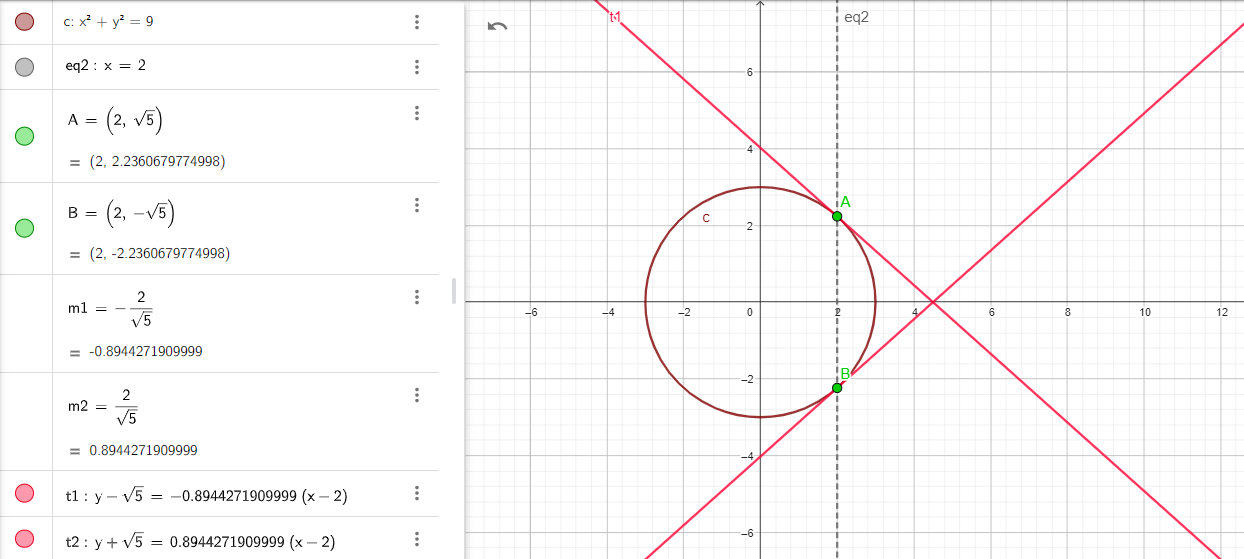
\includegraphics[width=0.8\textwidth]{./public/g1.png}
\end{figure}









% Tabla
\section*{Tabla de derivadas}
\begin{center}
	\noindent
	\begin{minipage}{0.5\textwidth}
		\centering
		\begin{tabular}{|>{\centering\arraybackslash}m{3.5cm}|>{\centering\arraybackslash}m{3cm}|}
			\hline
			Función           & Derivada                       \\
			\hline
			$(k)$ (constante) & $0$                            \\
			$x^n$             & $nx^{n-1}$                     \\
			$x^\frac{m}{n}$   & $\frac{m}{n}x^{\frac{m}{n}-1}$ \\
			$\sin(x)$         & $\cos(x)$                      \\
			$\cos(x)$         & $-\sin(x)$                     \\
			$\tan(x)$         & $\sec^2(x)$                    \\
			$\arcsin(x)$      & $\dfrac{1}{\sqrt{1-x^2}}$      \\
			$\arccos(x)$      & $-\dfrac{1}{\sqrt{1-x^2}}$     \\
			$\arctan(x)$      & $\dfrac{1}{1+x^2}$             \\
			$e^x$             & $e^x$                          \\
			$\ln(x)$          & $\dfrac{1}{x}$                 \\[10px]
			\hline
		\end{tabular}
	\end{minipage}%
	\begin{minipage}{0.5\textwidth}
		\centering
		\begin{tabular}{|>{\centering\arraybackslash}m{3.5cm}|>{\centering\arraybackslash}m{3cm}|}
			\hline
			$a^x$              & $a^x \ln(a)$                    \\
			$\log_b{x}$        & $\dfrac{1}{x \ln(b)}$           \\
			$\sin^{-1}(x)$     & $\dfrac{1}{\sqrt{1-x^2}}$       \\
			$\cos^{-1}(x)$     & $-\dfrac{1}{\sqrt{1-x^2}}$      \\
			$\tan^{-1}(x)$     & $\dfrac{1}{1+x^2}$              \\
			$\cot^{-1}(x)$     & $-\dfrac{1}{1+x^2}$             \\
			$\sec^{-1}(x)$     & $\dfrac{1}{|x|\sqrt{x^2-1}}$    \\
			$\csc^{-1}(x)$     & $-\dfrac{1}{|x|\sqrt{x^2-1}}$   \\
			$ax^n$             & $anx^{n-1}$                     \\
			$ax^{\frac{m}{n}}$ & $\frac{m}{n}ax^{\frac{m}{n}-1}$ \\
			$ax^{bx}$          & $abx^{bx} \ln(a)$               \\[9px]
			\hline
		\end{tabular}
	\end{minipage}
\end{center}

\end{document}
